\chapter{Hacheur 4 quadrants utilisé en traction ferroviaire}

% Sources : https://www.techniques-ingenieur.fr/base-documentaire/ingenierie-des-transports-th14/materiel-roulant-ferroviaire-42630210/tramways-c4442/performances-en-traction-et-en-freinage-c4442niv10003.html


\textit{La structure réversible de ce type de hacheur permet d’envisager son utilisation pour le pilotage de machines à courant continu en traction, là où la réversibilité est la plus intéressante à exploiter. Il est utilisé pour toutes les gammes de puissance, l’exemple donné ici étant celui d’un tramway.}

Le tramway est modélisé par une ``voiture'' motorisée par une machine à courant continu, elle-même pilotée par un hacheur réversible alimenté par une source continue parfaite (de type caténaire). Le schéma simplifié du dispositif est représenté sur la figure suivante et correspond aux grandeurs décrites ci-dessous.

\begin{figure}[H]
\centering
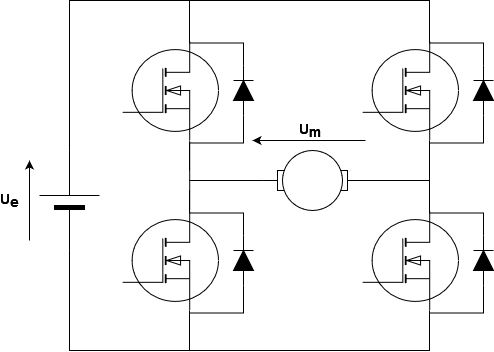
\includegraphics[width=0.55\linewidth]{TD_H4Q/fig/H4Q.png}
\caption{4 Quadrant chopper}
\end{figure}

Le hacheur est alimenté par une source de tension constante de valeur $U_E = 1500 V$. Il est constitué de deux bras de pont indépendants commandés à fréquence fixe $F_d = 2 kHz$. On note les rapports cycliques suivants : $\alpha_1$ pour $T_{11}$ et $\alpha_2$ pour $T_{21}$, la commande de chaque bras étant de type complémentaire. On suppose bien sûr les composants parfaits, diodes et transistors. Entre les deux bras de pont, on maintient la relation de commande suivante : $\alpha_1 + \alpha_2 = 1$.

Le moteur à courant continu est modélisé classiquement par sa f.e.m. $E$, sa résistance d’induit $R$ et son inductance d'induit $L$; son excitation est maintenue constante par un autre dispositif non étudié. La constante de couple (égale à la constante de f.e.m.) est notée $k_\varphi$ et les valeurs numériques sont les suivantes : 

$R = 0.2 \Omega$; $L = 25 mH$; $k_\varphi = 7.64 Nm/A$; vitesse nominale $N_n = 1500 tr/min$.

La voiture du tramway constitue la charge mécanique et présente, vis-à-vis de l’arbre moteur, un moment d’inertie $J = 200 kg.m^2$. En fonction du trajet, elle `` ramène'' également sur cet arbre moteur un couple résistant noté $C_v$.

\begin{enumerate}
\item \textbf{Commande complémentaire totale}

\begin{enumerate}
\item Représenter rapidement l'allure de la tension moteur $u_m(t)$ pour un rapport cyclique $\alpha_1$ quelconque, inférieur à $0.5$ puis supérieur à $0.5$.
\item Calculer la valeur moyenne de cette tension, notée $U_m$, en fonction de $\alpha_1$.
\end{enumerate}

\item\textbf{Description fonctionnelle}

On néglige dans cette partie l’ondulation du courant dans le moteur. De plus, un asservissement de courant supposé très rapide devant les constantes de temps mécaniques permet d’imposer la valeur souhaitée au courant d’induit du moteur, celle-ci étant notée $I_M$, constante.

\begin{enumerate}
\item Exprimer en fonction de $\alpha_1$, $U_E$ et $I_M$, les valeurs moyennes (à la fréquence de découpage $F_d$) de la tension aux bornes de l'induit moteur, notée $U_M$ et du courant absorbé par le hacheur à la source, noté $I_E$.
\item Le tramway s’arrête en côte (pente montante). Le poids de la voiture exerce alors un couple sur l’arbre moteur de valeur : $C_v$ de $382 Nm$. Quel est le rapport cyclique $\alpha_{10}$ nécessaire pour maintenir le tramway à l’arrêt ? Que vaut alors le courant $I_{E0}$ prélevé à la source d’alimentation (toujours en valeur moyenne) ?
\item Le tramway démarre à plat (on néglige le couple résistant) avec une accélération constante de $5 rad/s^2$ jusqu'à atteindre la vitesse de rotation nominale du moteur. 

\begin{enumerate}
\item Que vaut alors le courant moteur $I_m$ ?
\item Tracer l'évolution du rapport cyclique $\alpha_{1}$ lors de cette phase d'accélération.
\item Tracer l'évolution du courant $I_E$ prélevé à la source lors de cette phase d'accélération.
\item Calculer la durée d'accélération $\Delta t_a$.
\end{enumerate}

\item Le tramway effectue un trajet \textbf{en descente} à vitesse constante, le moteur tournant à sa vitesse nominale. Le poids exerce un couple $C_v$ de $382 Nm$. Que vaut le courant $I_{Ed}$ prélevé à la source d’alimentation ? Quel est alors la valeur du rapport cyclique $\alpha_{1d}$ permettant ce fonctionnement à vitesse constante ?
\item Freinage d’urgence en descente : lors du fonctionnement précédent (1.3), le conducteur demande un freinage d’urgence caractérisé par l’asservissement du courant d’induit à la valeur maximale tolérable par le hacheur et la machine, $I_{max} = 250 A$. On suppose que ce courant est imposé de façon quasi instantanée et reste présent lors de la phase de décélération, le couple lié au poids de la voiture étant toujours inchangé, égal à $382 Nm$.

\begin{enumerate}
\item Calculer et représenter l’évolution temporelle de la vitesse de rotation du moteur $\Omega(t)$, image de la vitesse du tramway.
\item Calculer la durée de ralentissement jusqu’à l’arrêt, notée $\Delta t_a$.
\item Déterminer lors de cette phase l’évolution du rapport cyclique $\alpha_1(t)$ en précisant notamment sa valeur au début du freinage et juste avant l’arrêt du véhicule.
\item Calculer l’énergie totale $E_C$ restituée à la source lors de ce freinage.
\end{enumerate}

\item Représenter les quadrants de fonctionnement du hacheur utilisés lors des différentes phases de fonctionnement du tramway.
\end{enumerate}

% \newpage
% \item \textbf{Commande complémentaire décalée du hacheur}

% On se propose ici de changer la commande des interrupteurs. Elle est réalisée suivant le schéma de la figure suivante. Pour chaque ``bras de pont'', la commande est toujours complémentaire de fréquence $F_d$ (on suppose que les commutations sont instantanées). Pour réaliser les modulations du rapport cyclique, on réalise la comparaison entre une modulatrice ($M_1$ ou $M_2$) et la tension image du rapport cyclique $\alpha$, notée $v_{alpha}$. On suppose que la sortie de ces comparateur est un signal binaire permettant de
% commander les interrupteurs.

% \begin{figure}[H]
% \centering
% 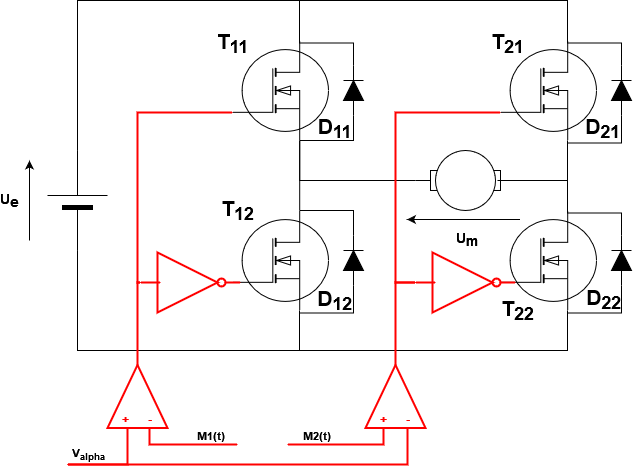
\includegraphics[width=0.6\linewidth]{TD_H4Q/fig/H4Q_decale.png}
% \caption{Shifted control of a 4 quadrant chopper}
% \end{figure}

% Les deux modulatrices sont représentées sur la figure suivante : il s’agit de signaux triangulaires en opposition de phase et d’amplitude $1 V$. Le signal $v_{alpha}$ est lui même d’amplitude maximale $1 V$, son amplitude réelle étant proportionnelle au rapport cyclique $\alpha$.

% \begin{enumerate}
% \item Pour $\alpha = 0.8$, représenter l’allure des fonctions de commutation $f_1(t)$ et $f_2(t)$ ainsi que la tension $u_m(t)$ aux bornes du moteur.
% \item Quelle est la fréquence de ce signal $u_m$ ? Quel est son ``rapport cyclique'', noté $\beta$ ?
% \item Pour $\alpha = 0.2$, représenter l'allure des fonctions de commutation $f_1(t)$ et $f_2(t)$ ainsi que la tension $u_m(t)$ aux bornes du moteur.
% \item Lorsque $\alpha$ est compris entre 0.5 et 1 et en négligeant la résistance $R$, déterminer l’ondulation $\Delta I_M$ du courant moteur. Quelle est sa valeur maximale $\Delta I_{M max}$?
% \item Quel est l’intérêt de cette commande par rapport à la commande complémentaire totale ?
% \end{enumerate}


% \newpage
% \begin{figure}[H]
% \centering
% 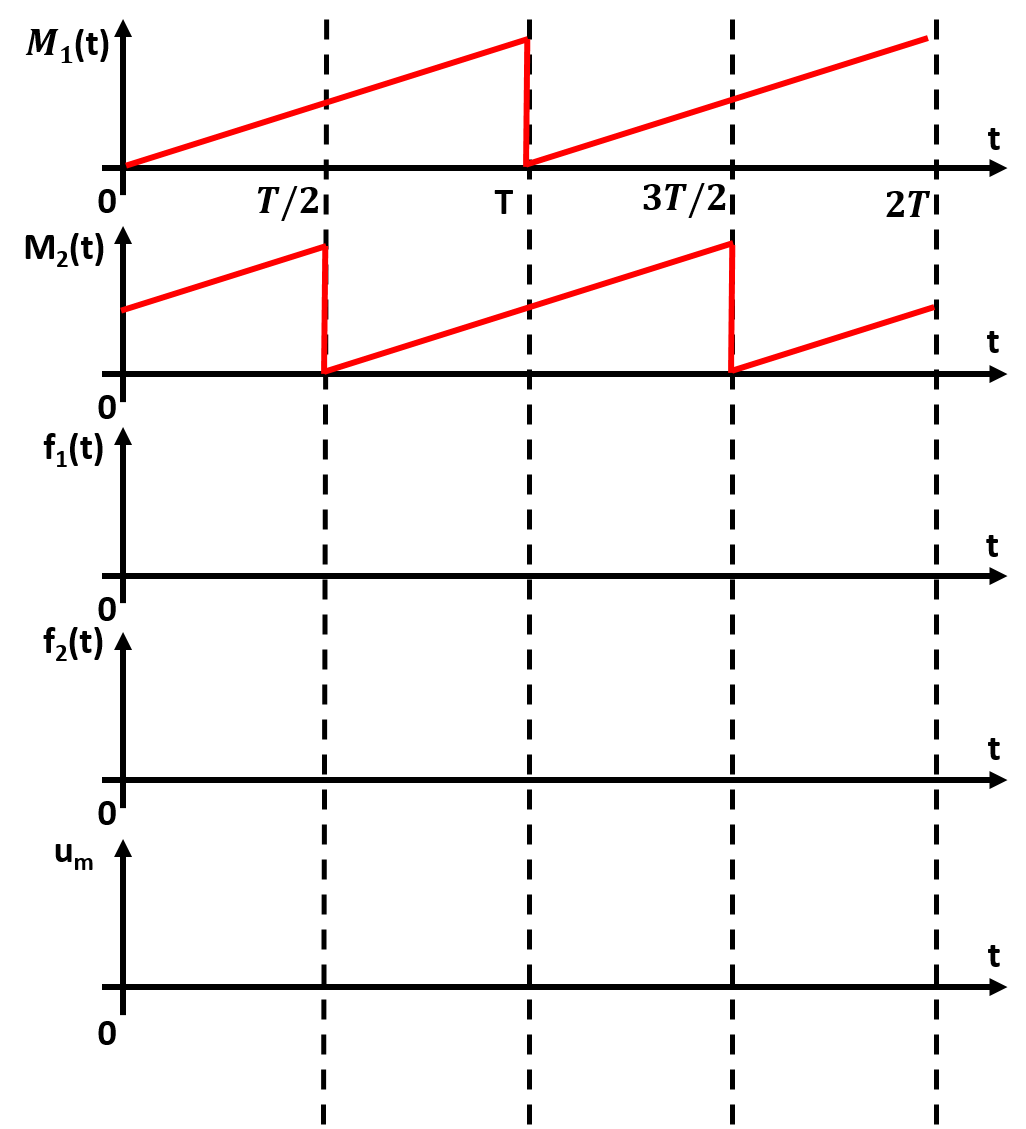
\includegraphics[width=\linewidth]{TD_H4Q/fig/answer.png}
% \caption{Shifted control of a 4 quadrant chopper}
% \end{figure}

%\newpage
%\item \textbf{Commande indépendante}
%
%On se propose ici de changer la commande des interrupteurs. Les transistors $T_{11}$ et $T_{12}$ sont toujours commandés de manière complémentaire avec le même signal que précédemment. les transistors $T_{21}$ et $T_{22}$ sont cette fois-ci commandés en fonction du signe de la tension de sortie souhaité : pour une tension $U_m$ positive, $T_{22}$ est fermé et $T_{21}$ est ouvert, et pour une tension $U_m$ négative, $T_{22}$ est ouvert et $T_{21}$ est fermé.
%
%\begin{figure}[H]
%\centering
%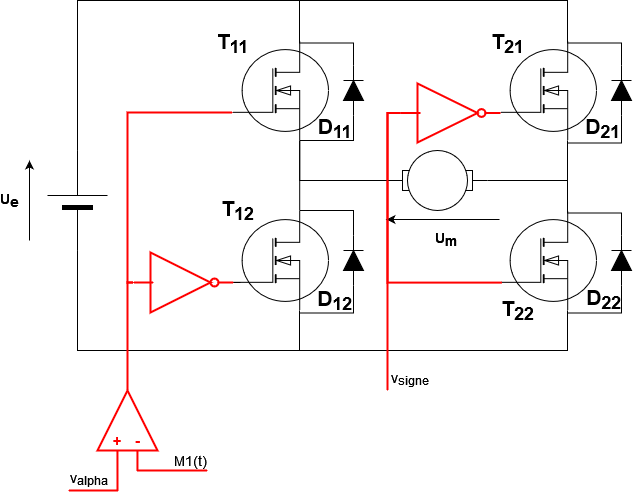
\includegraphics[width=0.6\linewidth]{TD_H4Q/fig/H4Q_indep.png}
%\caption{Independant control 4 quadrant chopper}
%\end{figure}
%
%\begin{enumerate}
%\item Représenter l'allure de $u_m(t)$ pour $\alpha=0.25$ et $v_{signe}=1$
%
%\item En déduire la relation entre la valeur moyenne de $u_m(t)$ et $\alpha$ lorsque $v_{signe}=1$
%
%\item Représenter l'allure de $u_m(t)$ pour $\alpha=0.25$ et $v_{signe}=0$
%
%\item En déduire la relation entre la valeur moyenne de $u_m(t)$ et $\alpha$ lorsque $v_{signe}=0$
%
%\item Conclure sur les avantages et inconvénients des différentes commandes
%\end{enumerate}
%
%\begin{figure}[H]
%\centering
%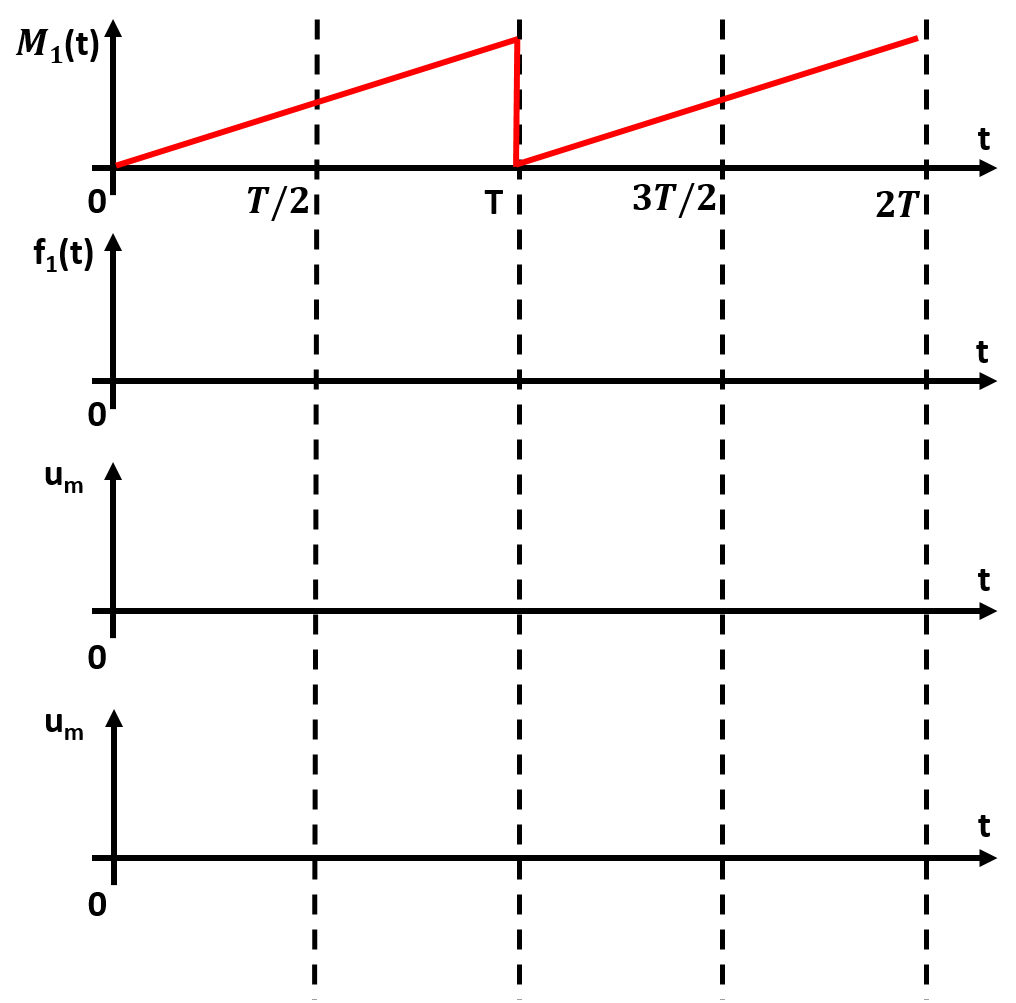
\includegraphics[width=\linewidth]{TD_H4Q/fig/answer2.png}
%%\caption{Shifted control of a 4 quadrant chopper}
%\end{figure}


\end{enumerate}


